In this section, we address two key problems outlined in the problem statement (Section 1.2):

\Paragraph{Redundant Work} One significant challenge arises when overlapping or identical range queries are executed in 
the database. The conventional approach performs the same amount of work for each query, involving a sort-merge 
operation across multiple levels to filter out invalid keys. However, a query-driven compaction strategy involves 
storing the result of the sort-merge operation from the initial range query at a higher level. By eliminating invalid 
keys at an earlier stage, subsequent overlapping range queries encounter reduced complexity. This leads to a more 
efficient execution, as later queries need to read fewer files, traverse fewer levels, and consequently encounter fewer 
invalid keys.

\Paragraph{Increased Write Amplification} The conventional method initiates compactions that retain invalid keys within 
the resulting SST files until they reach the last level, thereby causing a rise in write amplification. The query-driven
compaction strategy helps in eliminating invalid keys throughout the compaction process, resulting in a reduction of 
write amplification and a consequential enhancement in overall system efficiency.

The introduction of aggressive compactions during range queries may create gaps between levels and alter the tree shape. 
Paradoxically, this deformation proves advantageous for future ingestions, acting as a preventive measure against 
triggering cascading compactions. 

To substantiate these hypothesis, we conducted a series of experiments on an emulator, 
implementing the query-driven compaction approach. The results validated our expectations, demonstrating that queries 
following a query-driven compaction exhibited significantly improved speed. This optimization not only accelerates query 
execution but also enhances the overall efficiency of the ingestion process. To provide a more concrete understanding, 
we implemented the query-driven compaction approach on RocksDB and conducted a series of experiments to validate its 
performance in a real-world setting. The details of which are outlined below.

\subsection{Experimental Settings}
We ran our experiments on baremetal cloud instances provided by Chameleon. We used `compute skylake' machines to run all 
our experiements.

\begin{itemize}
    \item CPU(s)\:: 48 Cores
    \item RAM\:: 187 GiB
    \item RocksDB version\:: 8.5.0
\end{itemize}

\subsection{Experimental Results}
First set of experiements that we ran were based on our first approach, where each range query has to 
perform query-driven compaction without thinking about the number of entries overlapping between levels. The workload that
we used is as follows.
\begin{enumerate}[leftmargin=*,labelindent=0mm, itemsep=0.2\baselineskip]
    \item Number of Inserts \-- 500000
    \item Number of Updates \-- 250000, 500000, 750000
    \item Number of Range Queries \-- 100 
    \item Selectivity for Range Queries \-- 0.2, 0.4, 0.8
\end{enumerate}

\begin{figure}
    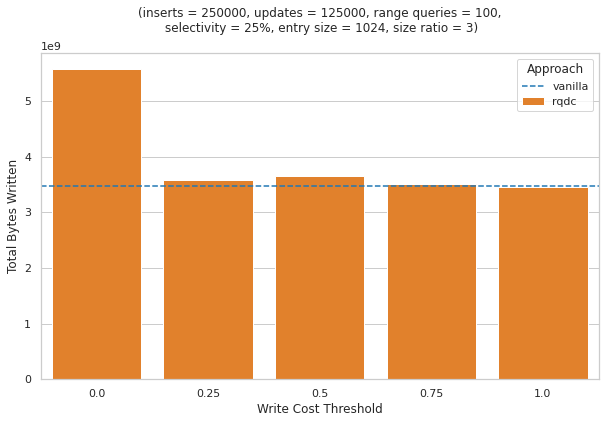
\includegraphics[scale=0.33]{Figures/utl_ltu_approach.png}
    \caption{Total write amplification in vanilla vs RQDC}\label{fig:utl_ltu_approach}
\end{figure}

The results show that the number of compactions triggered during the execution of the entire workload was significantly 
lower in the query-driven compaction than the vanilla approach (shown in Figure~\ref{fig:compaction_times}). This is 
expected since the query-driven approach performed these compactions during the range query executions. Additionally, 
the bytes written during background compactions are comparatively much less in our approach than in the vanilla approach
(shown in Figure~\ref{fig:compaction_write_bytes}) for the same reason. The Figure~\ref{fig:range_query_flush_write_bytes} 
shows the sum of bytes written during the ingestion of new keys and the bytes written during the query-driven compaction, 
which is almost 10x higher than the vanilla approach. The positive aspect is that this factor can be tuned by pre-computing 
the overlapping entries in the lower levels before performing the range query. If the lower levels have fewer entries 
that overlap with the higher level, then we can perform the vanilla fashion range query. However, if the overlap is more, 
then we can opt for query-driven compaction. These first set of experiments gave us a clear indication that we cannot 
use the query-driven approach for each range query blindly.

% \begin{figure*}
%     \begin{subfigure}{0.33\textwidth}
%         \centering
%         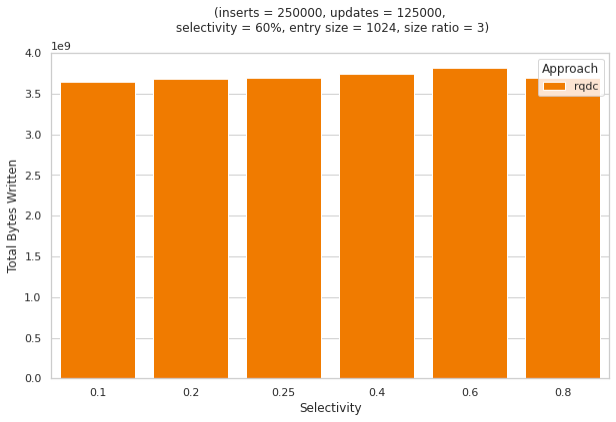
\includegraphics[width=\linewidth]{Figures/utl_ltu_with_varing_selectivity.png}
%         \caption{Total write amplification}\label{fig:utl_ltu_varing_selectivity}
%     \end{subfigure}%
%     \begin{subfigure}{0.33\textwidth}
%         \centering
%         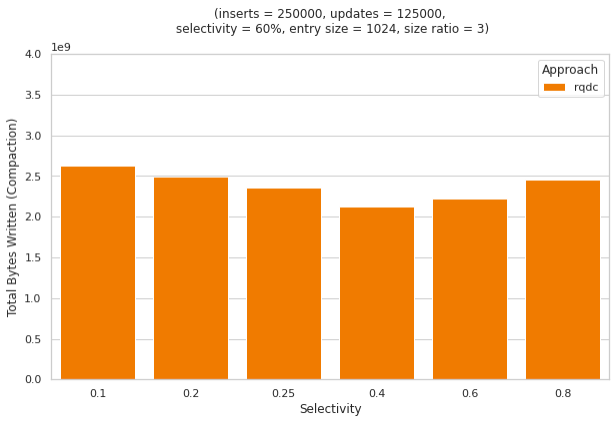
\includegraphics[width=\linewidth]{Figures/utl_ltu_varing_selectivity_compactions.png}
%         \caption{Compactions writes}\label{fig:utl_ltu_compaction_writes}
%     \end{subfigure}%
%     \begin{subfigure}{0.33\textwidth}
%         \centering
%         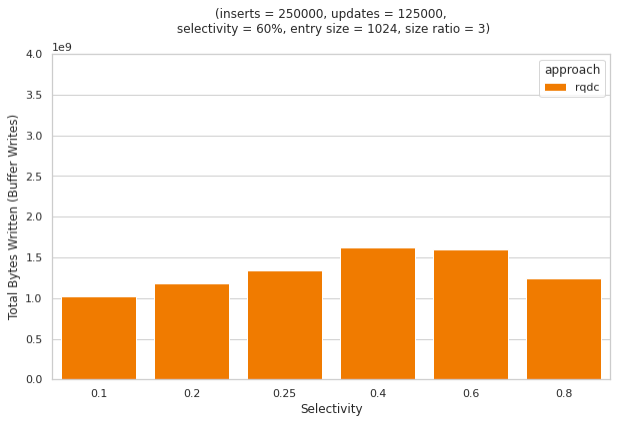
\includegraphics[width=\linewidth]{Figures/utl_ltu_varing_selectivity_flush.png}
%         \caption{Buffer writes}\label{fig:utl_ltu_buffer_writes}
%     \end{subfigure}
% \end{figure*}

\begin{figure}
    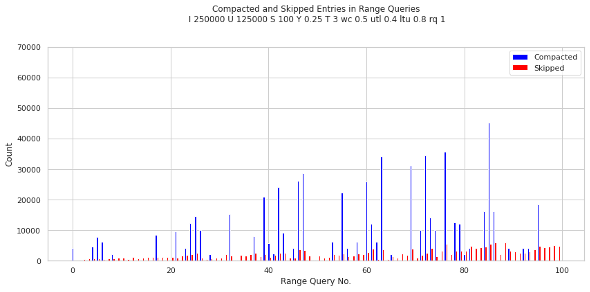
\includegraphics[scale=0.75]{Figures/compacted_vs_skipped.png}
    \caption{Compacted vs skipped keys during compaction}\label{fig:compacted_vs_skipped}
\end{figure}

We ran our second set of experiments using more informative compaction approach that we dicussed in section 4.3. The 
observations are as follows: the new approach has nearly the same write amplification as we have for vanilla but 
additionally provides a small benefit of reduced space amplification. The experiments were conducted for different $UTL$ and $LTU$ 
thresholds for a 25\% selectivity of range queries (shown in Figure~\ref{fig:utl_ltu_approach}). When the threshold is 
$0.0$, the compactions are performed blindly without thinking about the ovalapping entires.

% We also ran experiements with varying selectivites for the same number of range queries and found a slight bell curve for the write 
% amplications (shown in Figure~\ref{fig:utl_ltu_varing_selectivity},\ \ref{fig:utl_ltu_compaction_writes},\ \ref{fig:utl_ltu_buffer_writes}). 
% This was interesting, showing that for larger selectivities, the query-driven approach performs fewer compactions and 
% falls back to doing vanilla range queries because most of the data is already compacted due to previous range query compactions.

From these experiments we also observed that query-driven compaction compacts fairly large number of valid entries for the size ratio 3 (shown 
in Figure~\ref{fig:compacted_vs_skipped}). This might suggest that workloads benefiting from query-driven compaction 
should have more frequent updates, and the size ratio should be considerably larger. A smaller size ratio aids in 
promptly removing invalid keys as soon as updates are executed. This leads us to the next set of experimental design.

Our third set of experimental design was as follows: we ran the experiment in 11 epochs. The first epoch consisted only 
of inserts, set at 1 million to ensure our database was fully loaded. Subsequently, we ran 10 epochs with 25\% updates 
and 100 range queries of varying selectivities (10\% to 80\%). After each epoch, we recorded the total number of bytes 
written up to that point, the time taken by each range query in that epoch, and the total number of files and keys in 
our database. 

This set of experiments yielded promising results, as shown in Figure~\ref{fig:epoch_experiments}. The query-driven 
compaction approach wrote fewer bytes in every epoch after the 8th epoch. The level stats also showed that our approach 
had fewer files and fewer entries than vanilla. It removed a significant number of logically invalid entries during the 
compactions performed with range queries. This indicates that the query-driven approach outperformed the vanilla 
approach in terms of write and space amplification. This solves our second problem that we discussed above, namely 
``Increased Write Amplification''. 

\begin{figure}
    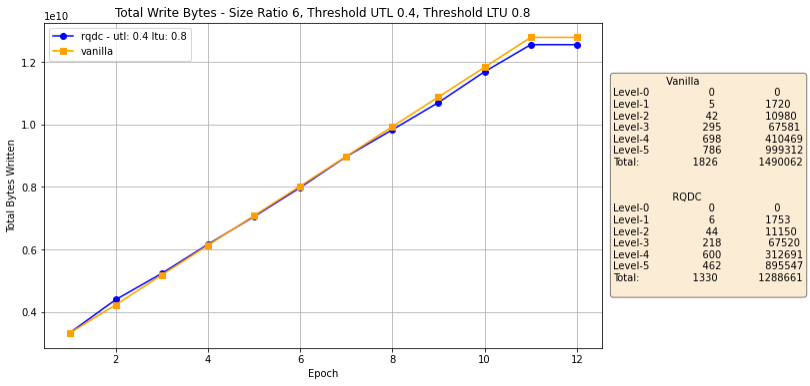
\includegraphics[scale=0.55]{Figures/epoch_experiments.png}
    \caption{Epoch experiments}\label{fig:epoch_experiments}
\end{figure}

\begin{figure}
    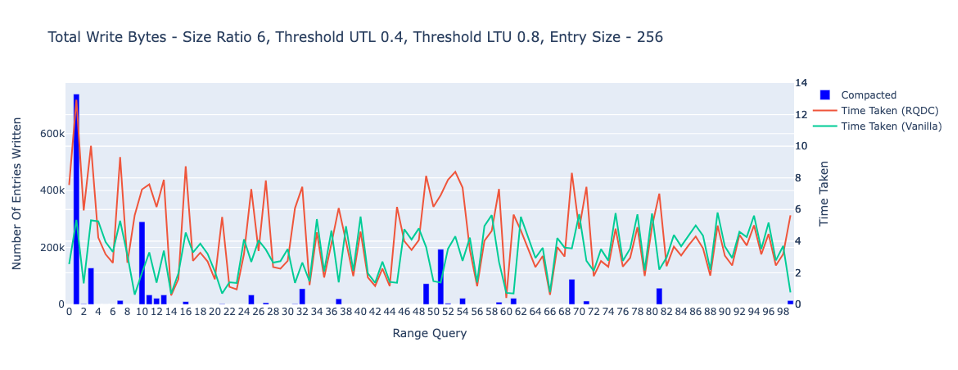
\includegraphics[scale=0.52]{Figures/first_epoch.png}
    \caption{First epoch updates and range queries}\label{fig:first_epoch}
\end{figure}

\begin{figure}
    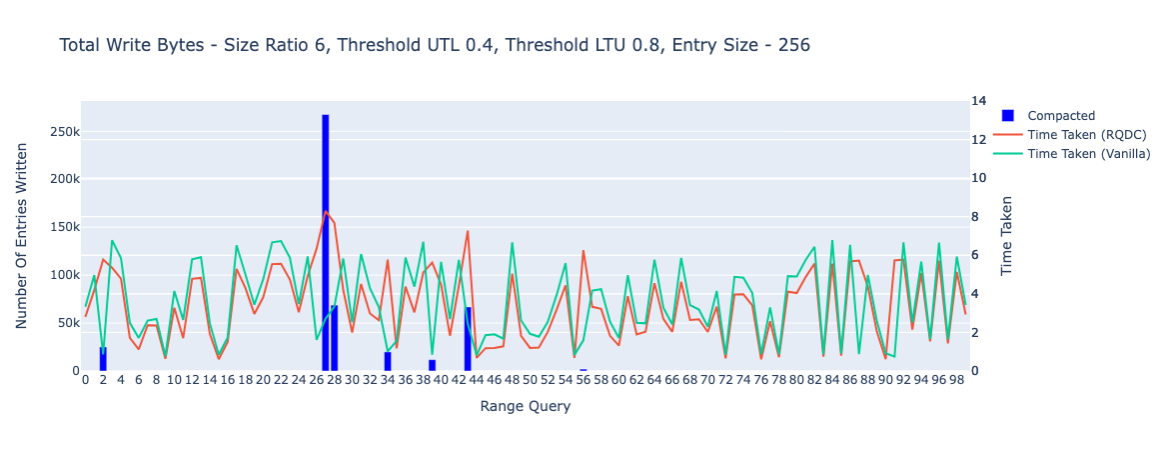
\includegraphics[scale=0.42]{Figures/last_epoch.png}
    \caption{Last epoch updates and range queries}\label{fig:last_epoch}
\end{figure}

We also observed the pattern of query-driven compaction through all of our epochs. The first epoch will have more 
opportunity to do the compactions since the lower levels are fully compact. The query driven compaction will take more 
time to perform the range query because of extra work performed with range query. The vanilla will take less time but 
stores more invalid keys to its levels. In the last few epochs the query-driven compaction will take less time to 
perform range queries because it will read few bytes than vanilla. We have shown the first and last epochs in 
Figure~\ref{fig:first_epoch},\ \ref{fig:last_epoch}.

Since we removed the invalid keys during the query-driven compaction, the subsequent range queries triggered after a 
successful execution of query-driven compaction will read fewer invalid keys (assuming the range is overlapping), 
leading to faster execution. This addresses our first problem of performing redundant work. Now, if the same range 
query is executed again, it may read only valid keys from the database.

% \begin{figure}
%     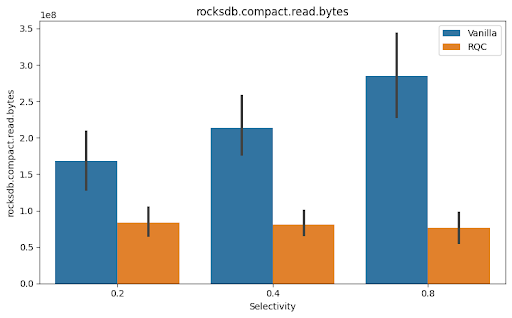
\includegraphics[scale=0.45]{Figures/Compaction Read Bytes.png}
%     \caption{Number of bytes read during compactions}\label{fig:compaction_read_bytes}
% \end{figure}

% Figure-\ref{fig:compaction_read_bytes} \& Figure-\ref{fig:compaction_write_bytes} shows the comparison between read and 
% writes bytes during the compactions that were triggered in vanilla and query-driven comapactions. We can see that the 
% bytes that were read and written during the vanilla are much higher than the newer approach

% \begin{figure}
%     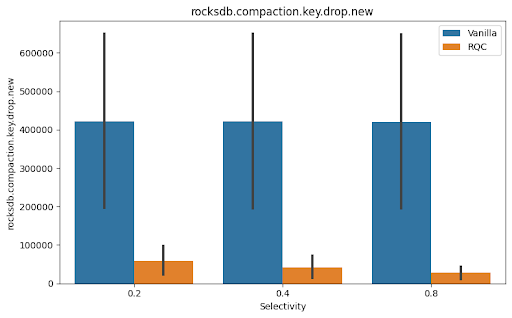
\includegraphics[scale=0.45]{Figures/Keys Drop In Compactions.png}
%     \caption{Number of keys dropped during compactions}\label{fig:keys_drop_in_compactions}
% \end{figure}

% Figure-\ref{fig:keys_drop_in_compactions} shows the number of keys that were dropped or re-written with newer values 
% while compaction.

% \begin{figure}
%     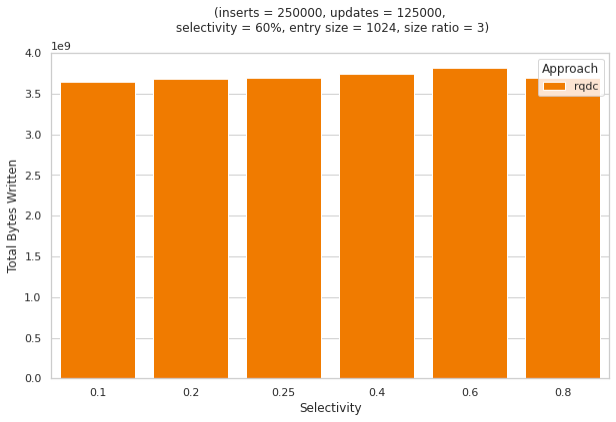
\includegraphics[scale=0.7]{Figures/utl_ltu_with_varing_selectivity.png}
%     \caption{Total write amplification in varing selectivity}\label{fig:utl_ltu_varing_selectivity}
% \end{figure}

% \begin{figure}
%     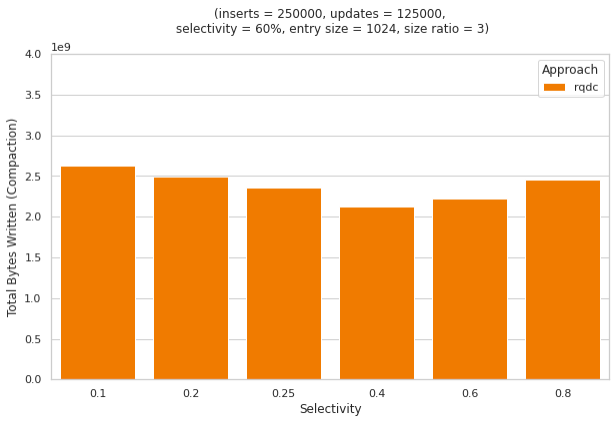
\includegraphics[scale=0.7]{Figures/utl_ltu_varing_selectivity_compactions.png}
%     \caption{Compactions writes in varing selectivity}\label{fig:utl_ltu_compaction_writes}
% \end{figure}

% \begin{figure}
%     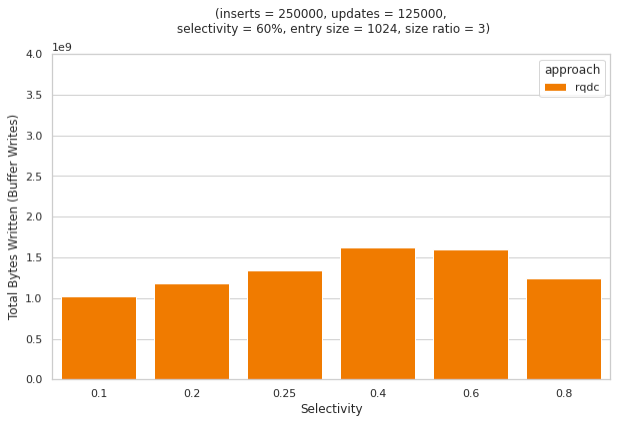
\includegraphics[scale=0.7]{Figures/utl_ltu_varing_selectivity_flush.png}
%     \caption{Buffer writes in varing selectivity}\label{fig:utl_ltu_buffer_writes}
% \end{figure}
